\documentclass{beamer}
\usepackage{tikz}

% internal parameters
\usetheme{Copenhagen}
\usecolortheme{default}
\setbeamertemplate{caption}[numbered]

% packages
\usepackage{graphics}
\usepackage{amsmath}
\usepackage{xcolor}
\usepackage{physics}
\usepackage{fontawesome}
\usepackage{mathrsfs}  
\usepackage{multirow}


\title[Wobbling Motion, NSP-2022]{Evaluation of the Wobbling Motion in Even-Even Nuclei Within a Simple Rotor Model}
\author[Robert, POENARU]{Robert POENARU\inst{1,2}}

\institute[VFU]
{
  \inst{1}%
  Doctoral School of Physics @ UB\\
  Bucharest, Romania
  \and
  \inst{2}%
  Dept. of Th. Phys. @ IFIN-HH\\
  Magurele, Romania
}

\date{\textit{International Conference on Nuclear Structure Properties}\\\textit{\today}}


\expandafter\def\expandafter\insertshorttitle\expandafter{%
  \insertshorttitle\hfill%
  \insertframenumber\,/\,\inserttotalframenumber}
%------------------------------------------------------------
\begin{document}
%---------------------------------------------------------
\frame{\titlepage}
\begin{frame}
  \frametitle{Table of Contents}
\end{frame}

\begin{frame}{Nuclear Deformation}
  \begin{itemize}
    \item Most of the nuclei are either \emph{spherical} or \emph{axially symmetric} in their ground-state.
    \item Deformation parameter $\beta$ (\textit{Bohr, 1969}): preserves axial symmetry
  \end{itemize}
  \begin{figure}
    \centering
    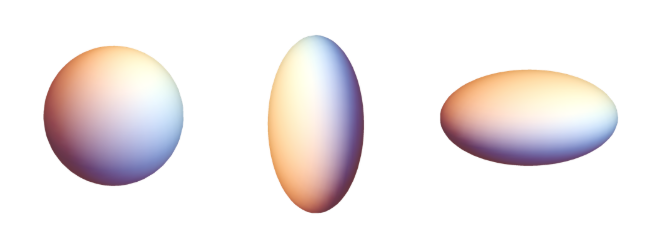
\includegraphics[width=0.99\textwidth]{Figs/nuclear_shapes.png}
    \caption{\textbf{spherical:} $\beta=0$\ \textbf{prolate:} $\beta>0$\ \textbf{oblate:} $\beta<0$}
  \end{figure}
\end{frame}

\begin{frame}
  \frametitle{Nuclear Triaxiality}
  \begin{alertblock}{Non-axial shapes}
    \begin{itemize}
      \item Deviations from symmetric shapes can occur across the chart of nuclides $\to$ \textbf{triaxial nuclei}.
      \item The triaxiality parameter $\gamma$ (\textit{Bohr, 1969}): departure from axial symmetry
    \end{itemize}
  \end{alertblock}
  \begin{figure}
    \centering
    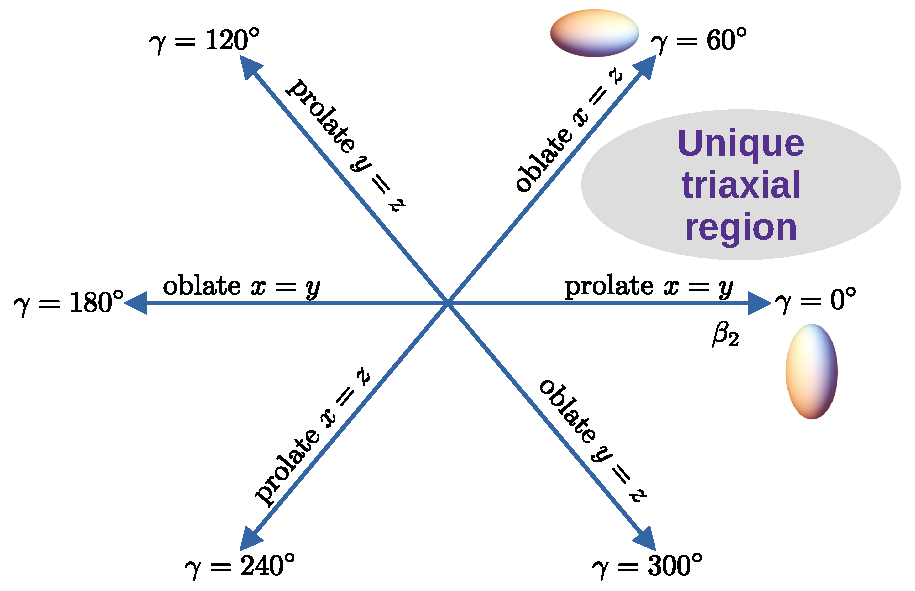
\includegraphics[scale=0.42]{Figs/nice_diagram.pdf}
    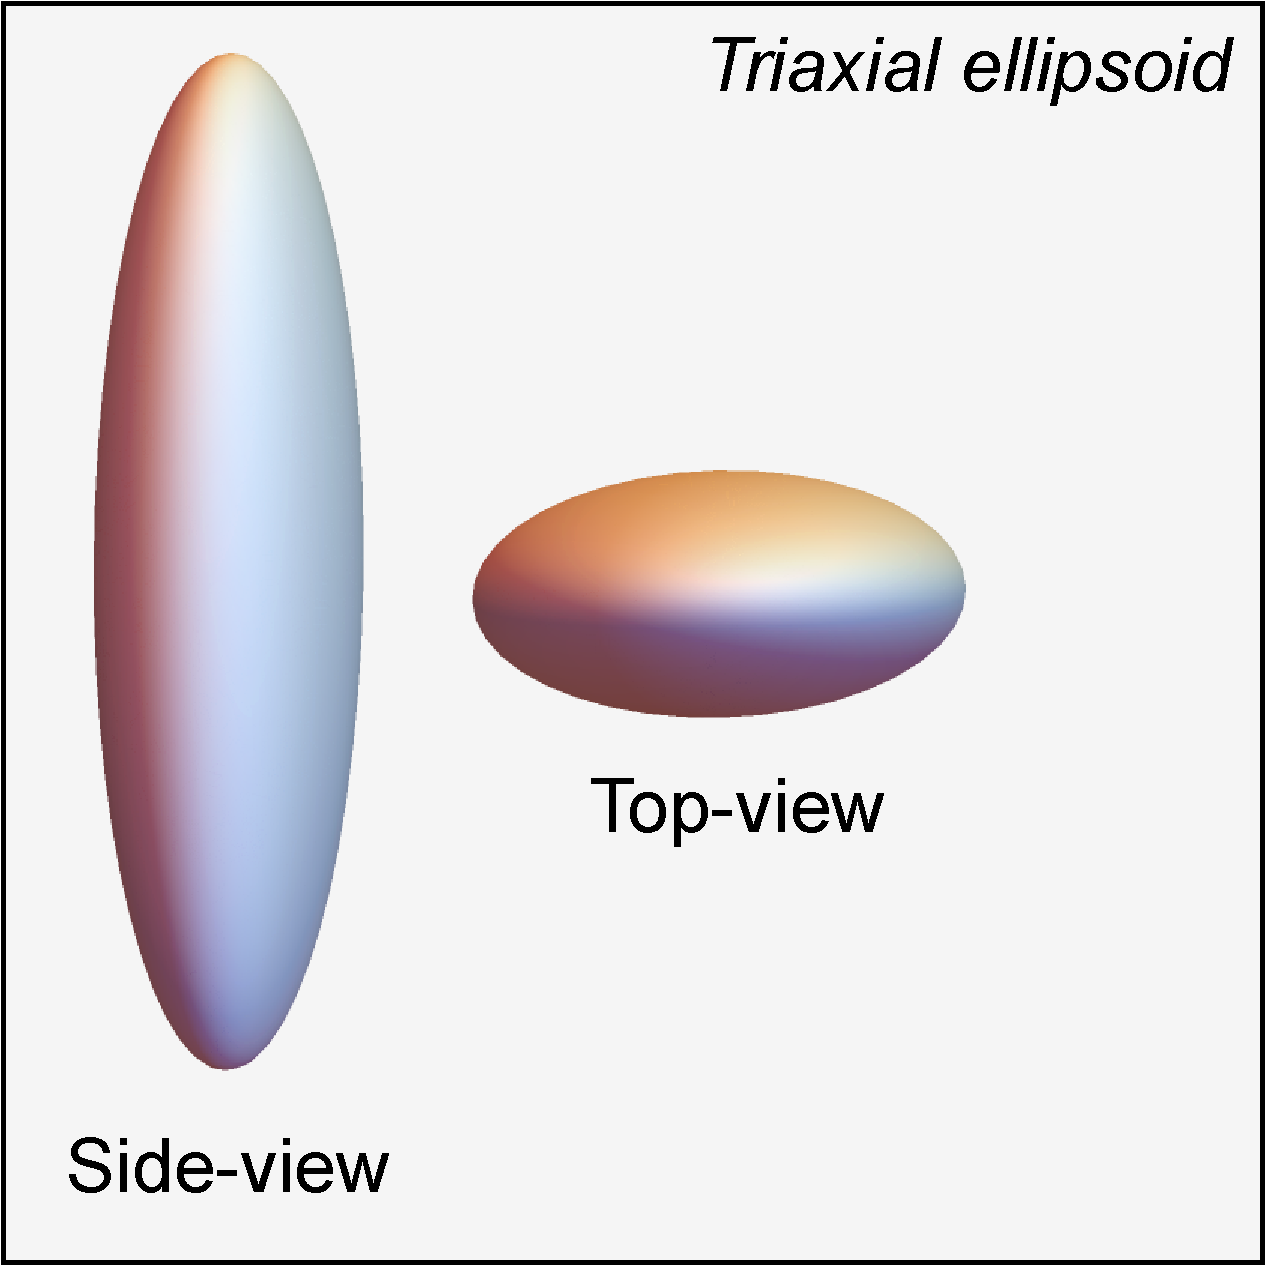
\includegraphics[scale=0.19]{Figs/triaxial-shape.pdf}
    % \caption{The $(\beta,\gamma)$ plane divided into six equivalent parts, depicting nuclear surfaces.}
  \end{figure}
\end{frame}

\begin{frame}
  \frametitle{Fingerprints for Triaxiality}
  \begin{itemize}
    \item Stable triaxial nuclei represent a real challenge for experimentalists and theoreticians
    \item Clear signatures for confirming stable triaxiality in nuclei
    \begin{enumerate}
      \item Chiral symmetry breaking (\textit{Frauendorf, 1997})
      \item \textbf{Wobbling motion} (\textit{Bohr \& Mottelson, 1975})
    \end{enumerate}
  \end{itemize}
  \begin{block}{Wobbling Motion (WM)}
    \begin{itemize}
      \item Unique to non-axial nuclei
      \item Predicted 50 years ago for even-$A$ nuclei (i.e., the simple wobbler)
      \item First experimental evidence for $^{163}$Lu (\textit{Ødegård}, 2001)
      \item Currently confirmed wobblers $A\approx[100,130,160,180]$.
    \end{itemize}
  \end{block}
\end{frame}

\begin{frame}
  \frametitle{Triaxial Rotor Energy}
  \begin{itemize}
    \item Rigid body rotational energy: $E_\text{rot}\propto\frac{\hbar^2}{2\mathcal{J}_\text{max}}I(I+1 )$
    \item A triaxial nucleus can rotate about any of the three axes $\rightarrow$ \emph{rich energy spectra} 
    \item MOI anisotropy $\rightarrow$ the \emph{main rotation} around $\mathcal{J}_\text{max}$ is disturbed by the other two axes  $\rightarrow$ \textbf{resulting motion of the rotating nucleus has an oscillating behavior}
  \end{itemize}
  \begin{figure}
    \centering
    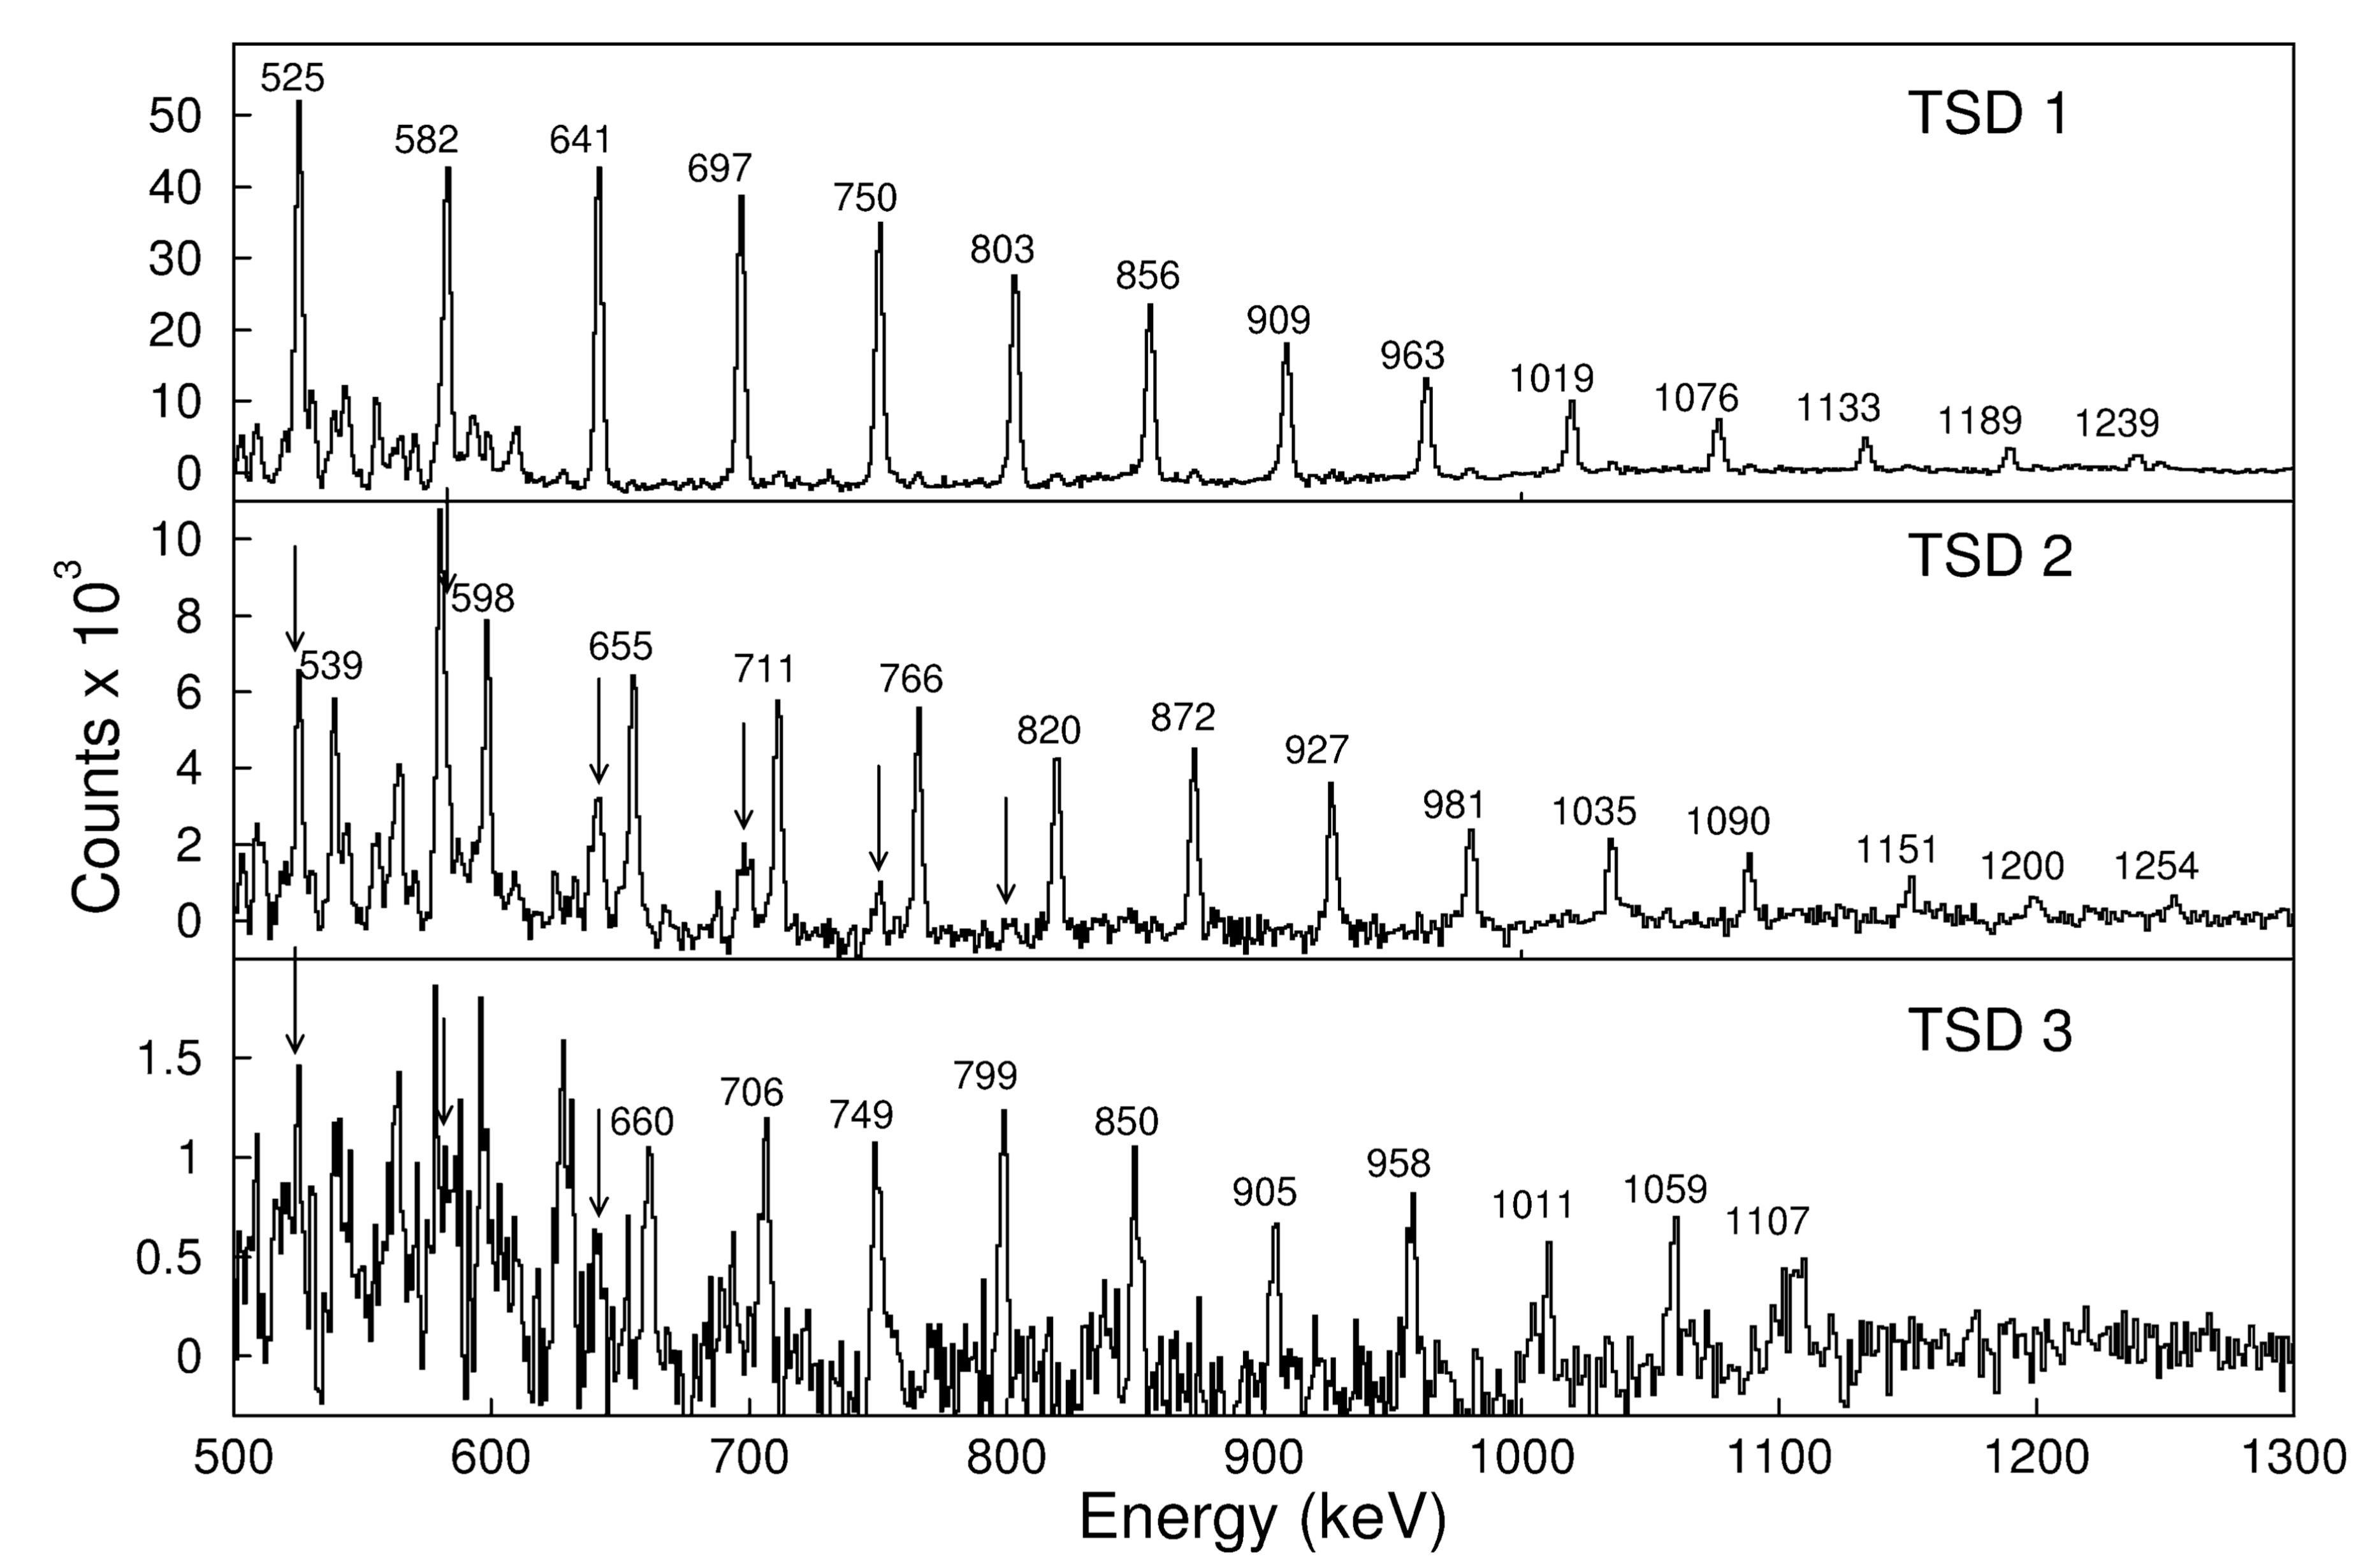
\includegraphics[scale=0.10]{Figs/collective-spectra.pdf}
    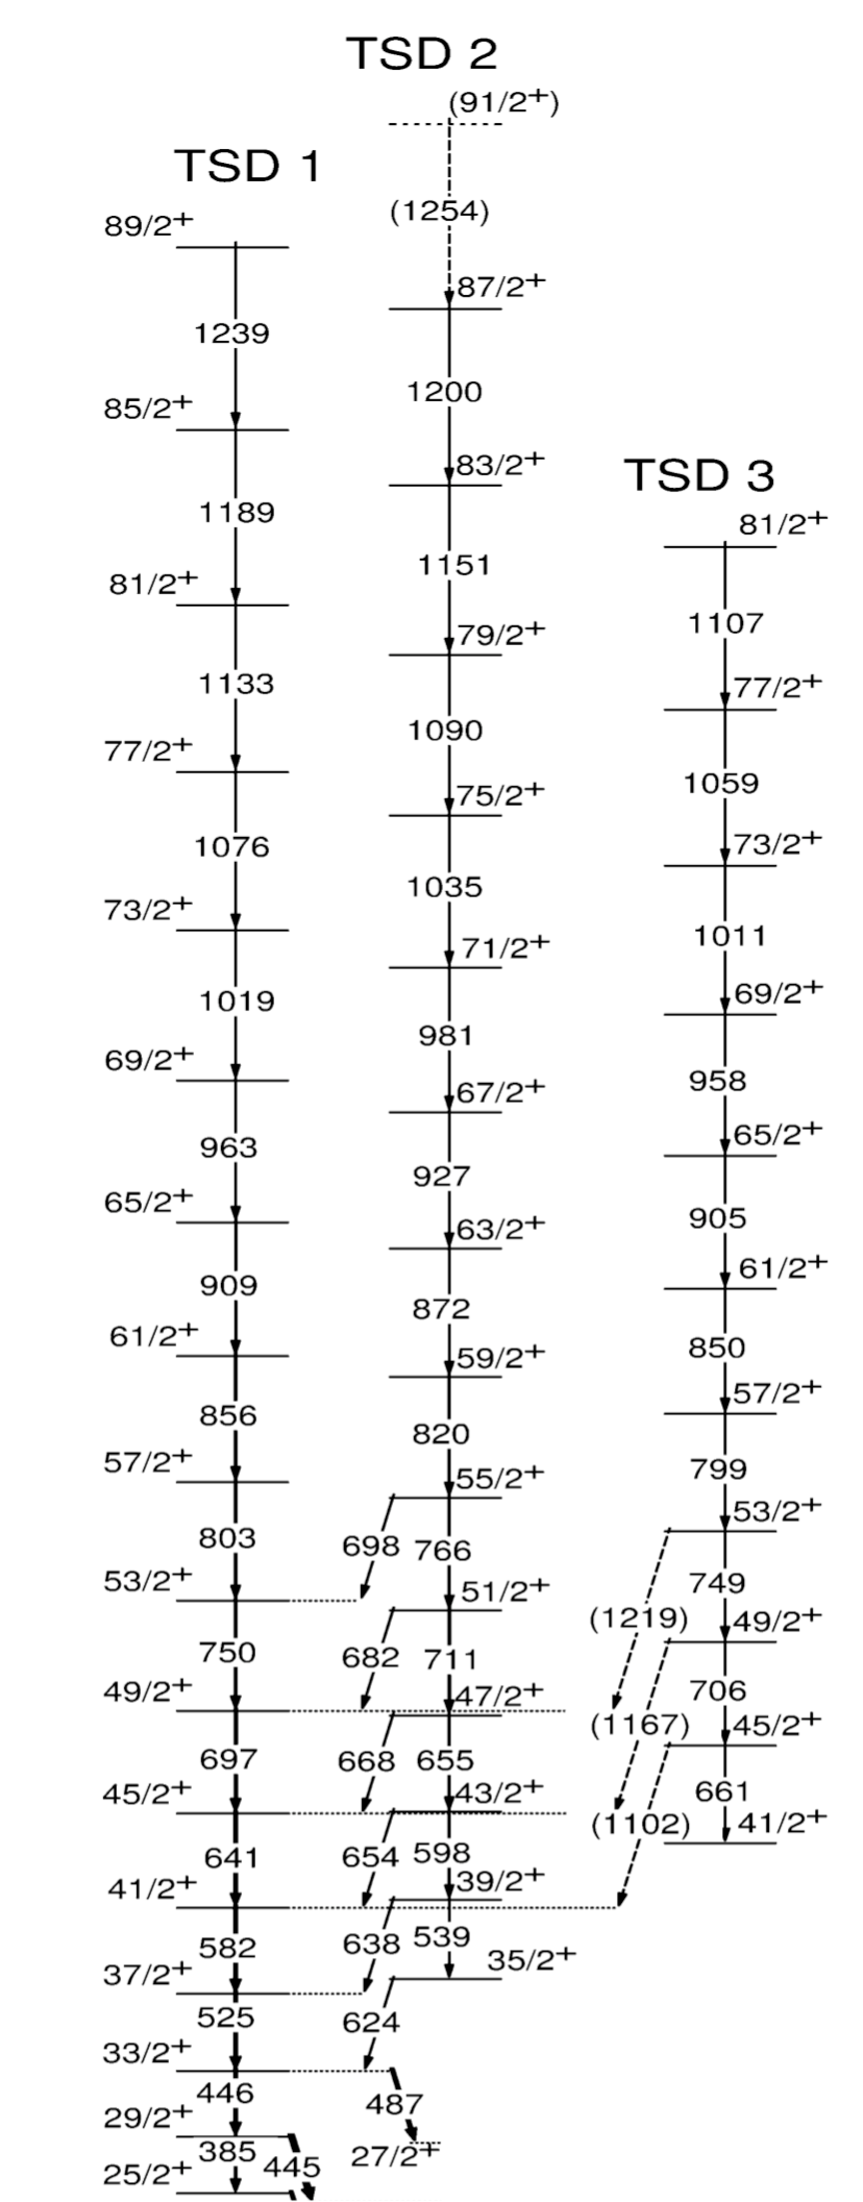
\includegraphics[scale=0.11]{Figs/collective-levels.pdf}
  \end{figure}
  \tiny{\textit{Figures from Schönwaßer et al., 2001}}
\end{frame}

\begin{frame}
  \frametitle{Wobbling Motion}
\begin{itemize}
  \item Oscillatory character of $\mathbf{I}$ $\rightarrow$ $\mathbf{I}$ \emph{disaligned} w.r.t. body-fixed axes
  \item The a.m. \textbf{precesses} and \textbf{wobbles} around the axis with $\mathcal{J}_\text{max}$
  \item The precession of $\mathbf{I}$ can increase by \textbf{tilting} 
  \item Tilting by an energy quanta $\sim$ \emph{vibrational character} $\rightarrow$ \textbf{wobbling phonon} $n_w=0,1,2...$
\end{itemize}
  \begin{figure}
    \centering
    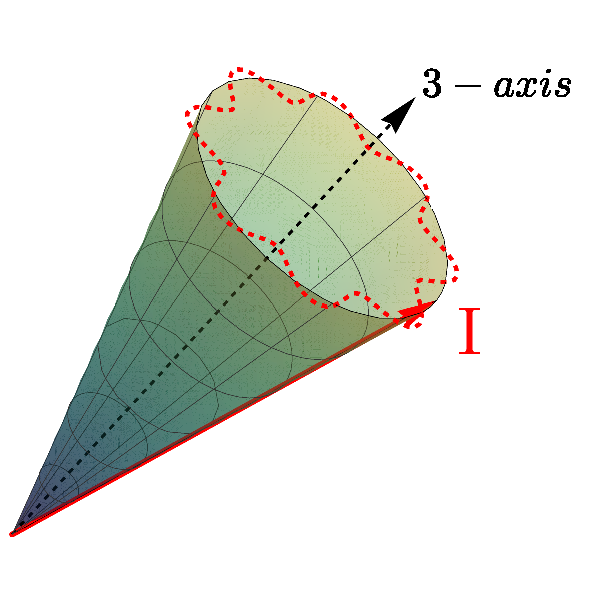
\includegraphics[scale=0.39]{Figs/precessional_cone_2.pdf}
    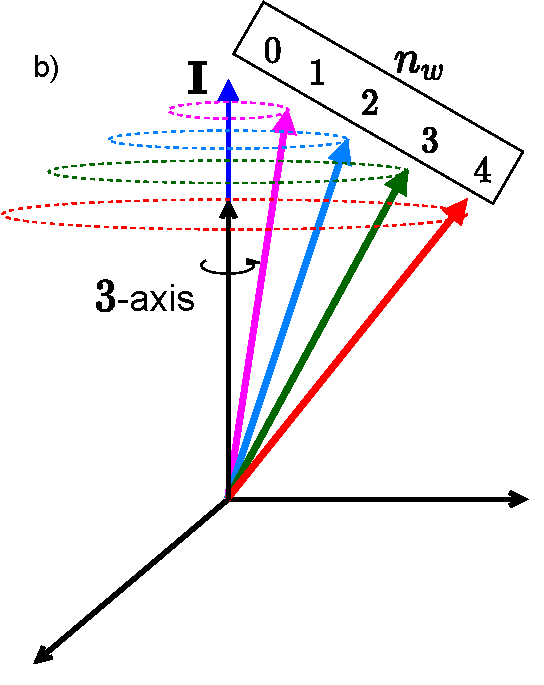
\includegraphics[scale=0.32]{Figs/wobbling_n_schematic-2.pdf}
    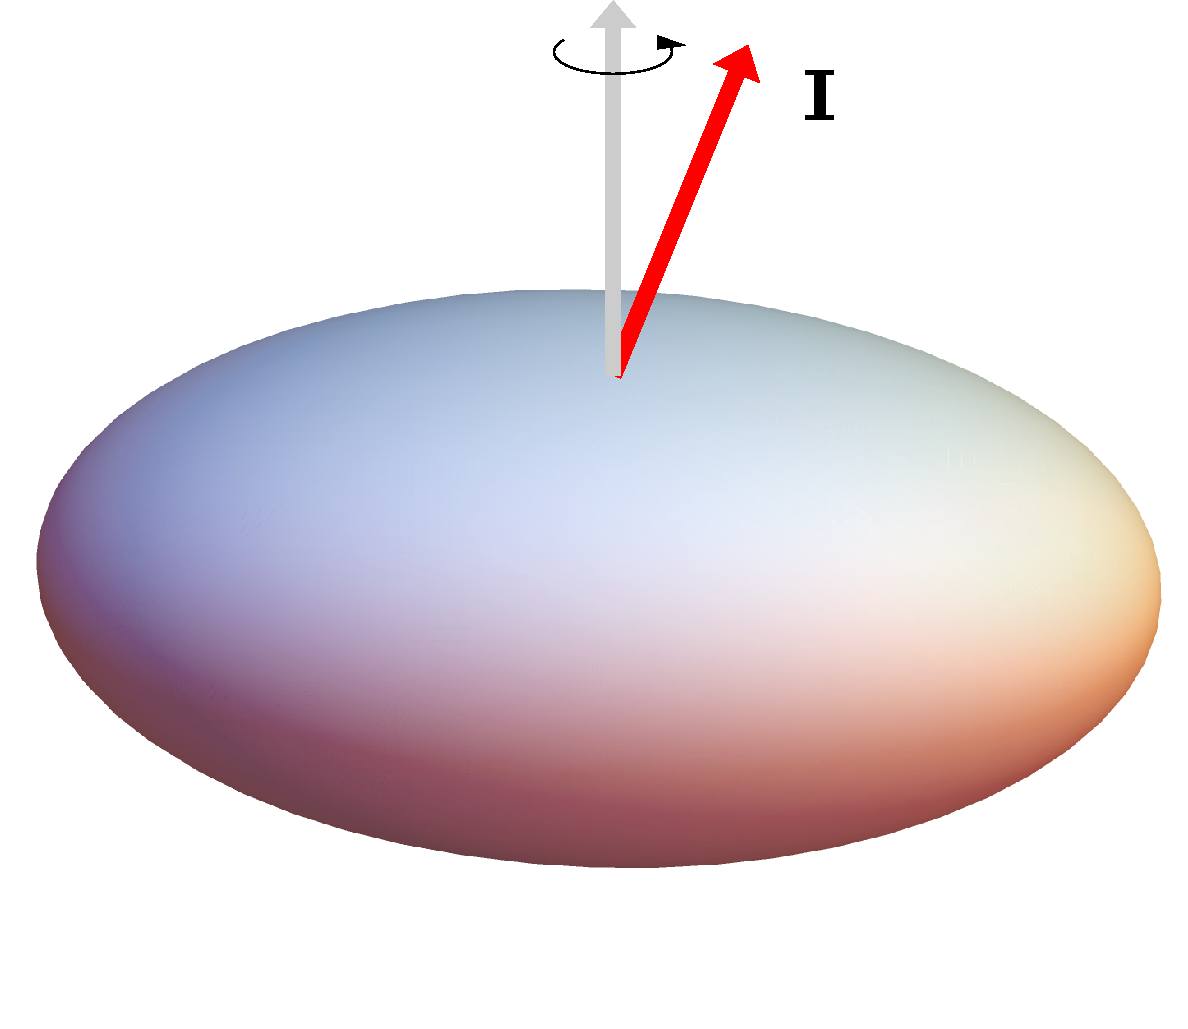
\includegraphics[scale=0.18]{Figs/triaxial-shapes-rotor-core.pdf}
  \end{figure}
\end{frame}

\begin{frame}
  \frametitle{Wobbling Spectrum}
\begin{block}{Even-$A$ Nuclei}
  \begin{itemize}
    \item Employing the Harmonic Approximation \textit{(Bohr, 1969)}
    \item $\hat{H}$ composed of a {\color{red}\emph{rotational}} part and {\color{blue}\emph{harmonic oscillation}} (i.e., wobbling) part:
  \end{itemize}
  \begin{align}
    \hat{H}={\color{red}\frac{\hbar^2}{2\mathcal{J}_\text{max}}I(I+1)}+{\color{blue}\hbar\omega_\text{wob}\left(n_w+\frac{1}{2}\right)}\ , n_w=0,1,2,\dots
    \label{wobbling-hamiltonian-even-A}
  \end{align}
\end{block}
\begin{figure}
  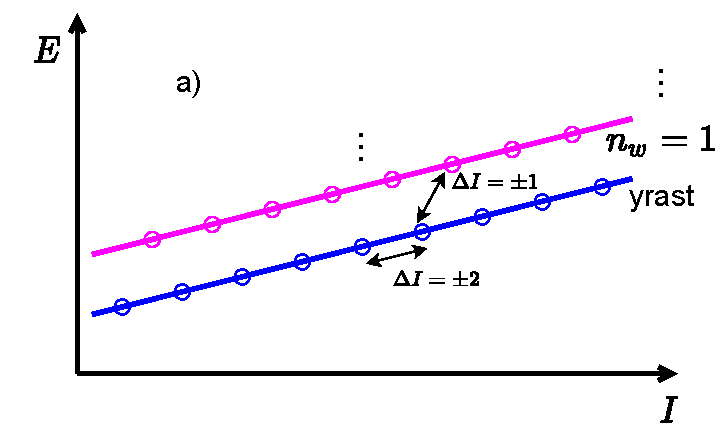
\includegraphics[scale=0.5]{Figs/wobbling_n_schematic-1.pdf}
  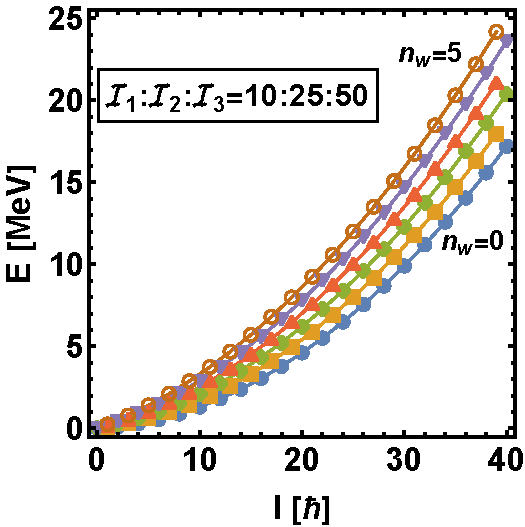
\includegraphics[scale=0.4]{Figs/wobblingFreq-evenA.pdf}
\end{figure}
\end{frame}

\begin{frame}
  \frametitle{Energy spectrum - simple wobbling}
  \begin{columns}
    \begin{column}{0.65\textwidth}
      % \begin{alertblock}{Harmonic Approximation}
        \begin{itemize}
          \item Employed an energy spectrum of harmonic type according to Eq. \ref{wobbling-hamiltonian-even-A}:
          \begin{align}
            E_{I}={\color{red}\frac{\hbar^2}{2\mathcal{J}_3}I(I+1)}+{\color{blue}\hbar\omega_\text{wob}\left(n_w+\frac{1}{2}\right)}\nonumber
          \end{align}
          \item $\hbar\omega_\text{wob}$ - \textbf{wobbling frequency} - linear dependence on $I$ (fixed MOI ordering $\mathcal{J}_3>\mathcal{J}_{1,2}$)
          \begin{align}
            {\color{blue}\hbar\omega_\text{wob}(I)=2f(\mathcal{J}_1,\mathcal{J}_2,\mathcal{J}_3)\cdot I}\nonumber
          \end{align}
        \end{itemize}
      % \end{alertblock}
    \end{column}
    \begin{column}{0.4\textwidth}
      \begin{figure}
        \begin{center}
          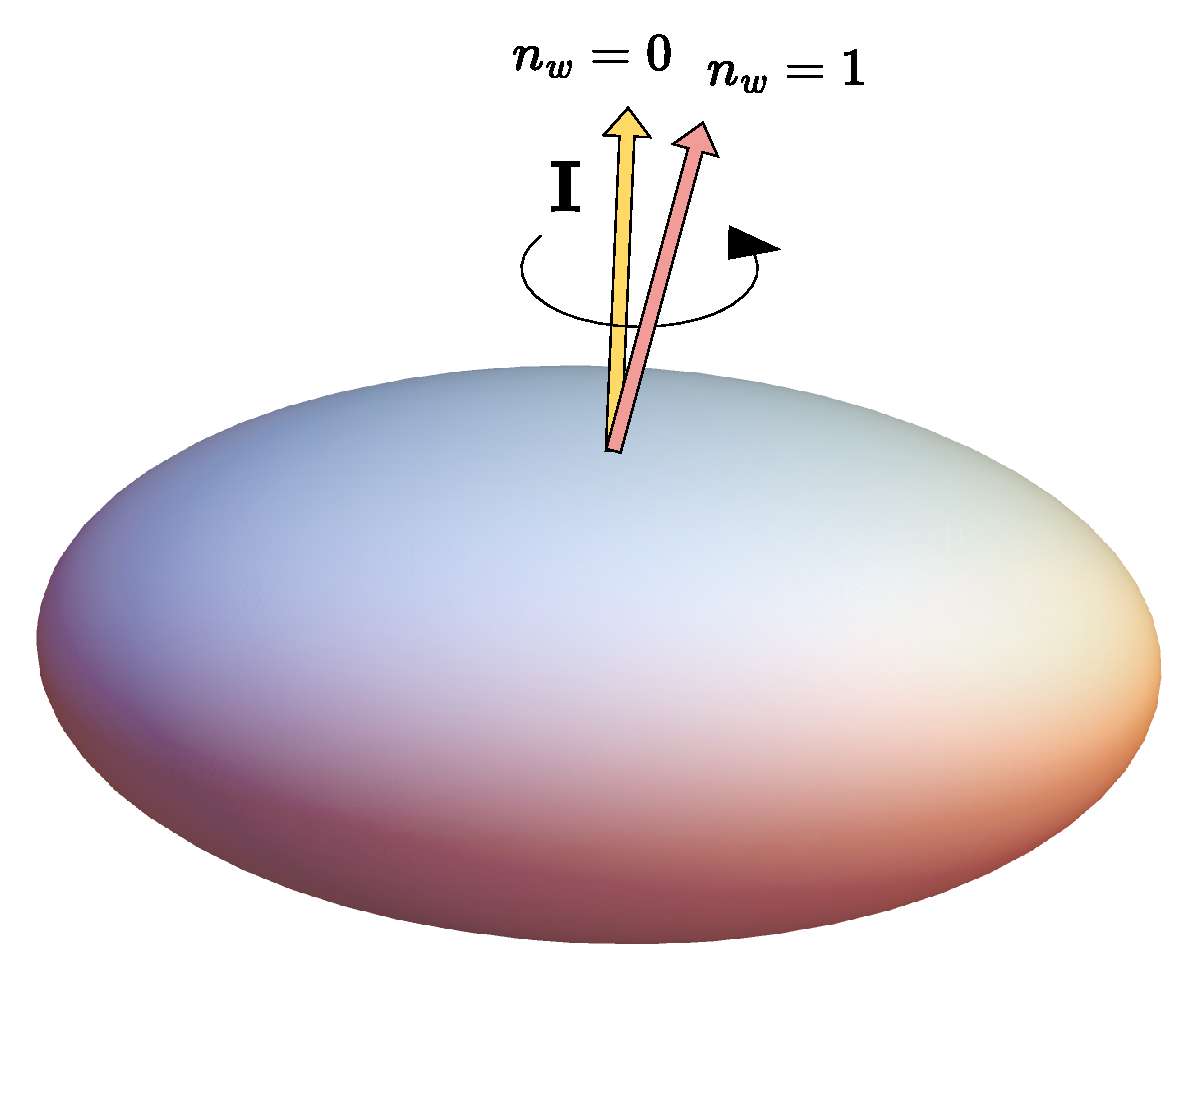
\includegraphics[scale=0.21]{Figs/triaxial-shapes-even-A.pdf}
        \end{center}
      \end{figure}
    \end{column}
  \end{columns}
\end{frame}

\begin{frame}
  \frametitle{New Results}
  \begin{itemize}
    \item New experimental measurements show \emph{potential} wobbling candidates in the $A\approx 130$ region
    \item Three even-$A$ are studied with the \emph{simple wobbler} formalism
    \begin{enumerate}
      \item $^{130}$Ba (\emph{Petrache et al. 2019})
      \item $^{134}$Ce (\emph{Petrache and Guo, 2016})
      \item $^{136}$Nd (\emph{Lv et al., 2018})
    \end{enumerate}
    \item Study the excited spectra: \emph{theoretical model checks the data?}
  \end{itemize}
\end{frame}

\begin{frame}
  \frametitle{Model}

  \begin{alertblock}{Harmonic Approximation}
    \begin{itemize}
      \item Reproduced the excited spectra for the wobbling bands
      \item Employ a \emph{free parameter set}: $\mathcal{P}=\left[\mathcal{J}_1,\mathcal{J}_2,\mathcal{J}_3\right]$
      \item Adopt a fitting procedure:
      \begin{align}
        \chi^2=\frac{1}{N_T}\sum_{i=1}^{N_T}\frac{\left(E_\text{exp}^{(i)}-E_\text{th}^{(i)}\right)^2}{E_\text{exp}^{(i)}}
      \end{align}
      \item $N_T\ \rightarrow$ total number of wobbling states within the nucleus
    \end{itemize}
  \end{alertblock}

\end{frame}

\begin{frame}
  \frametitle{New Results for 130Ba}
  \begin{minipage}{.8\textwidth}
    \begin{block}{Recent findings for even-even nuclei}
      \begin{itemize}
        \item Two wobbling bands have been identified experimentally in \textbf{$^\mathbf{130}$Ba} (\textit{Petrache et al., 2019})
        \item DFT+PRM description of the wobbling motion described the excited spectra (\textit{Chen et al., 2019})
        \begin{itemize}
          \item Reproduced experimental energies
          \item Obtained deformation parameters self-consistently
          \item Stable triaxiality for $\beta=0.24$ and $\gamma=21.5^\circ$
        \end{itemize}
      \end{itemize}
    \end{block}
  \end{minipage}%
  \begin{minipage}{.2\textwidth}
    \begin{figure}
      \centering
      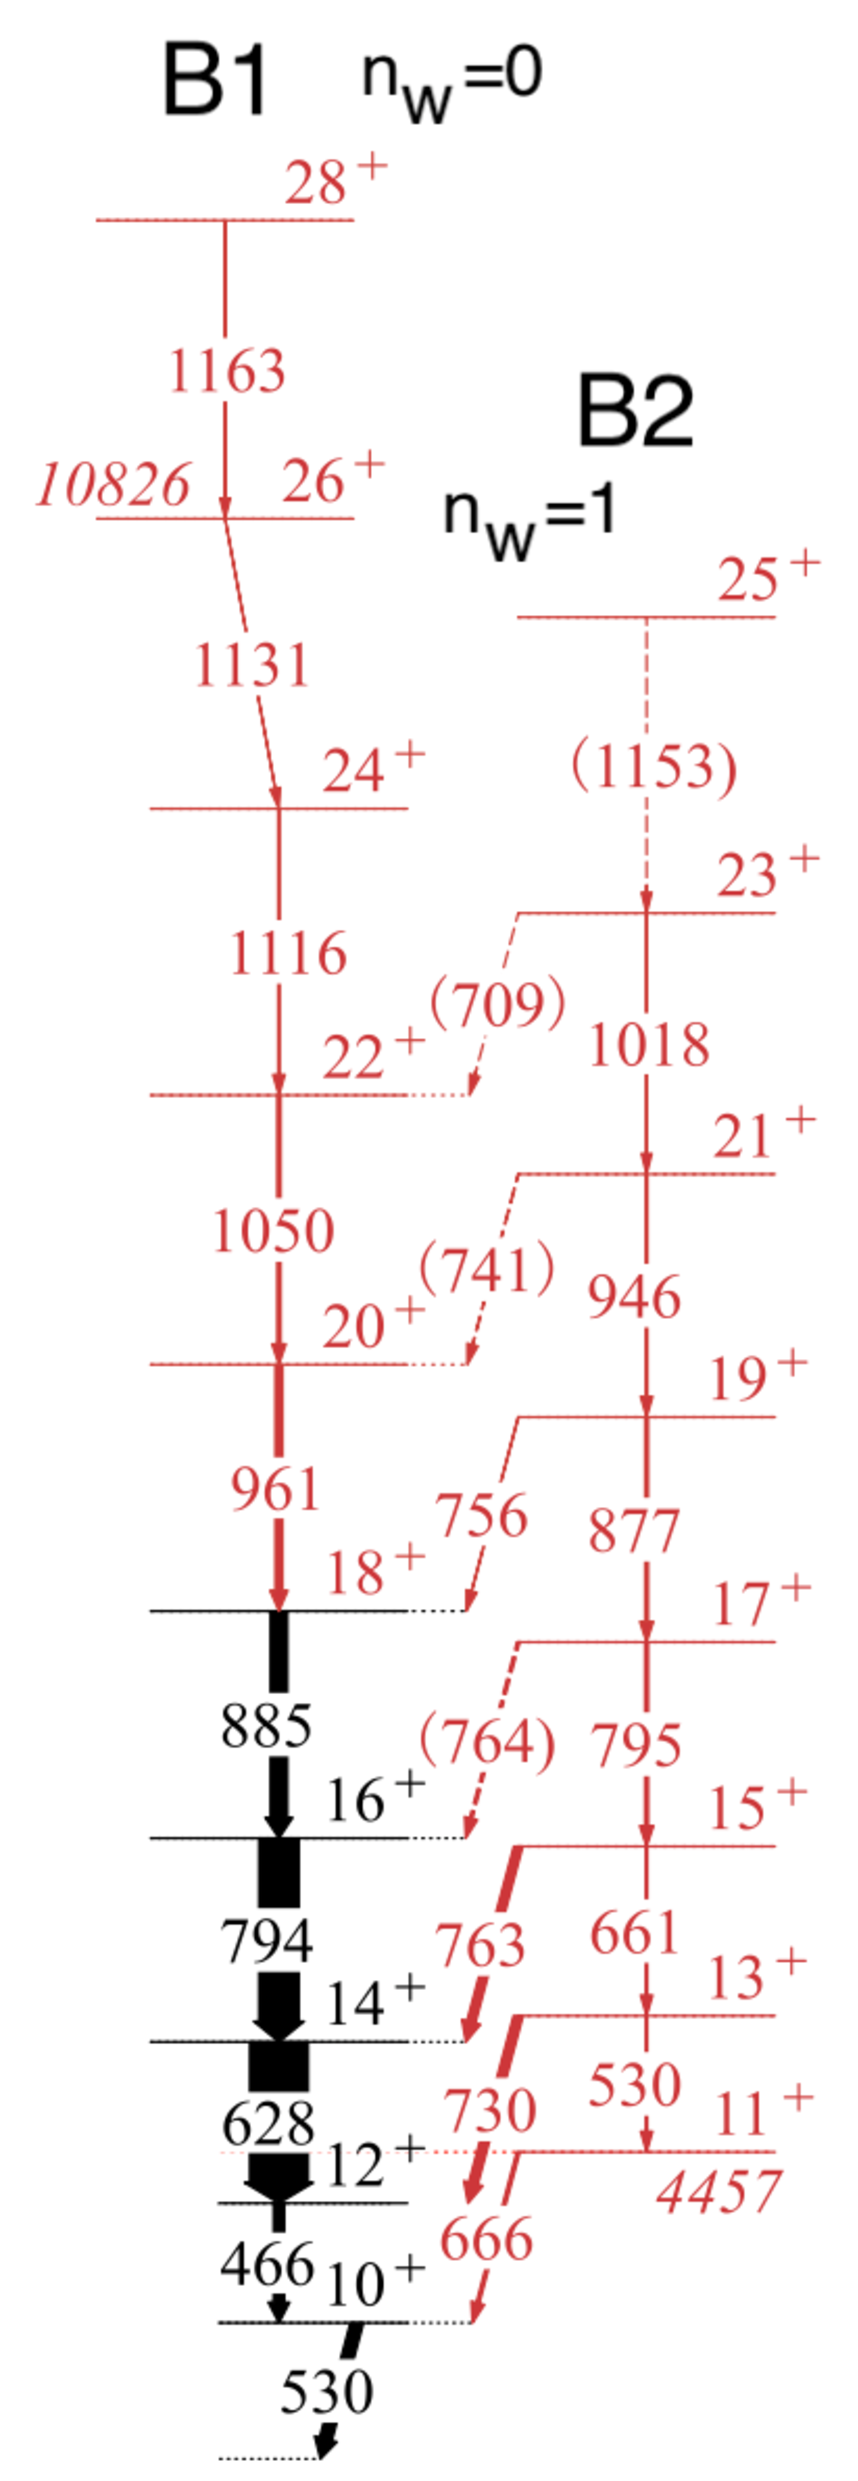
\includegraphics[scale=0.13]{Figs/ba-130-level-scheme.pdf}
      \tiny{\textit{Figure from Petrache et al., 2019}}
    \end{figure}
  \end{minipage}
\end{frame}

\begin{frame}
  \frametitle{New Results for 130Ba II}
  \begin{exampleblock}{Results for $^{130}$Ba \textbf{PRELIMINARY!}}
    \begin{table}
      \centering
      \begin{tabular}{|c|c|c|c|}
      \hline
      $\mathcal{J}_1^\text{fit}$ & $\mathcal{J}_2^\text{fit}$ & $\mathcal{J}_3^\text{fit}$ & \multirow{2}{*}{$\left[\hbar^2\text{MeV}^{-1}\right]$} \\ \cline{1-3}
      27                         & 22                         & $\mathbf{43}$                         &                                                       \\ \hline
      \end{tabular}
      \end{table}
      \begin{itemize}
        \item Maximal MOI is $\mathcal{J}_{3}>\mathcal{J}_{1,2}$
      \end{itemize}
\end{exampleblock}
\begin{figure}
  \centering
  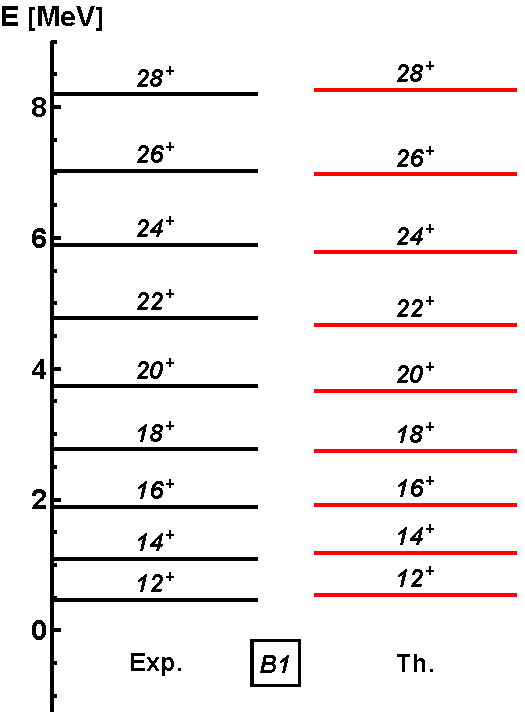
\includegraphics[scale=0.39]{Figs/ba130-band1.pdf}
  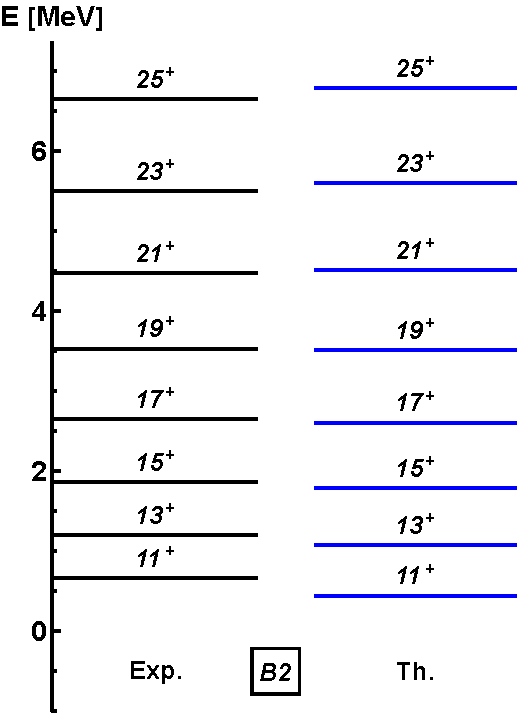
\includegraphics[scale=0.39]{Figs/ba130-band2.pdf}
\end{figure}
\end{frame}

\begin{frame}
  \frametitle{Electromagnetic Transitions 130Ba}

\begin{itemize}
  \item In the harmonic approximation, the three MOI are used to determine $B(E2)_\text{out}$
  \item $\beta_2$ and $\gamma$ are taken from Chen et al. $\rightarrow$ $(\beta,\gamma)=0.24,21.5^\circ$ $\rightarrow$ used to calculate the quadrupole components $Q_20$ and $Q_22$
  \item $B(E2)_\text{out}(I)=\frac{5}{16\pi}I^{-1}\left(\sqrt{3}Q_{20}\cdot f(\mathcal{J})+\sqrt{2}Q_{22}\cdot g(\mathcal{J})\right)$
\end{itemize}
\begin{columns}
\begin{column}{0.3\textwidth}
  \begin{table}
    \centering
    \resizebox{\textwidth}{!}{%
    \begin{tabular}{|c|ccc|}
      \hline
      \multirow{2}{*}{$I$} & \multicolumn{3}{c|}{$B(E2)_\text{out}/B(E2)_\text{in}$}                          \\ \cline{2-4} 
      & \multicolumn{1}{c|}{Th.} & \multicolumn{1}{c|}{PRM*} & Exp. \\ \hline
      11                   & \multicolumn{1}{c|}{0.37}       & \multicolumn{1}{c|}{-}           & -             \\ \hline
      13                   & \multicolumn{1}{c|}{0.32}       & \multicolumn{1}{c|}{0.51}       & 0.32         \\ \hline
      15                   & \multicolumn{1}{c|}{0.27}       & \multicolumn{1}{c|}{0.42}       & 0.36         \\ \hline
      17                   & \multicolumn{1}{c|}{0.24}       & \multicolumn{1}{c|}{0.35}       & 0.22         \\ \hline
      19                   & \multicolumn{1}{c|}{0.21}       & \multicolumn{1}{c|}{0.29}       & 0.22         \\ \hline
      21                   & \multicolumn{1}{c|}{0.19}       & \multicolumn{1}{c|}{0.25}       & 0.41         \\ \hline
      23                   & \multicolumn{1}{c|}{0.18}       & \multicolumn{1}{c|}{-}           &  -            \\ \hline
      25                   & \multicolumn{1}{c|}{0.16}       & \multicolumn{1}{c|}{-}           &  -            \\ \hline
    \end{tabular}%
    }
  \end{table}
\end{column}
\begin{column}{0.7\textwidth}
  \begin{figure}
    \centering
    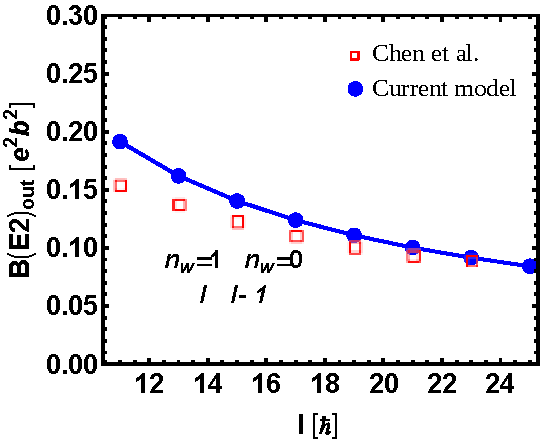
\includegraphics[scale=0.5]{Figs/ba130-EM.pdf}
  \end{figure}
  \end{column}
\end{columns}
\end{frame}

\begin{frame}
  \frametitle{New Results for 134Ce}
\begin{columns}
  \begin{column}{0.4\textwidth}
    \begin{figure}
      \centering
      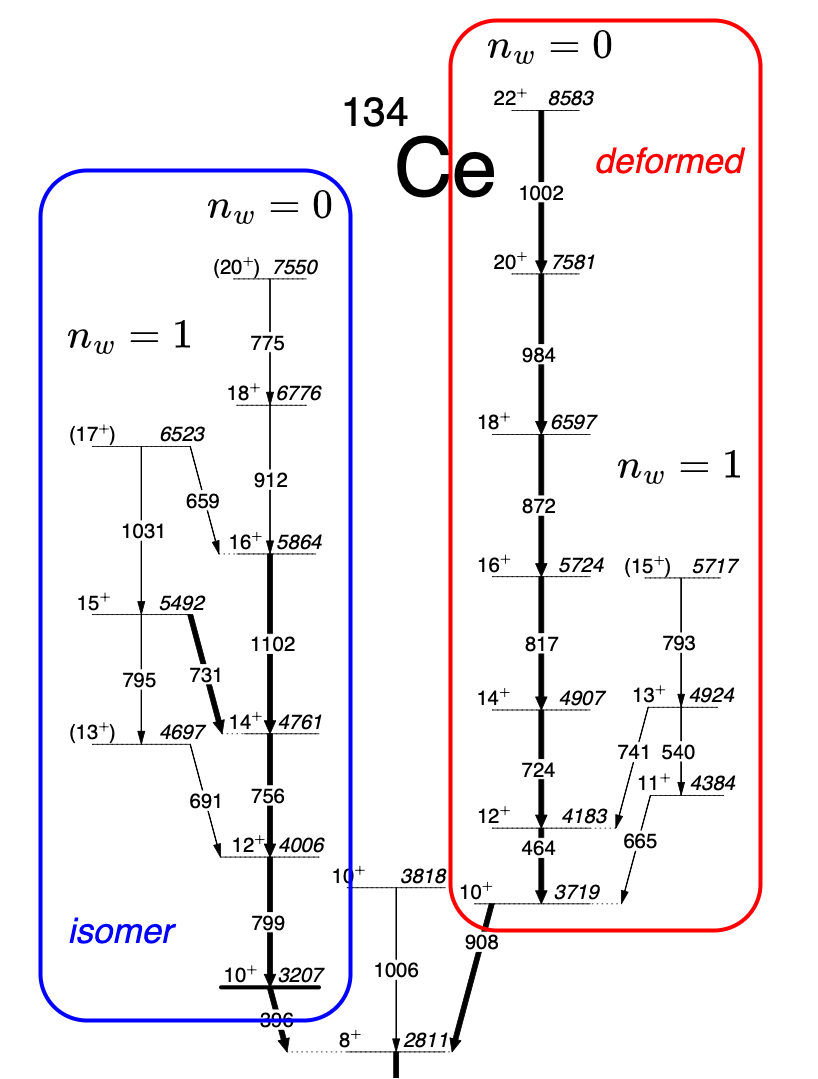
\includegraphics[scale=0.15]{Figs/triaxial-shapes-ce-134.png}
    \end{figure}
  \end{column}
  \begin{column}{0.6\textwidth}
    \begin{itemize}
      \item Petrache et al. found two sets of wobbling bands in $^{134}$Ce
      \item Wobbling confirmed in odd-$A$ $^{135}$Pr by Matta et al. 2015 $\rightarrow$ \emph{even-$A$ neighbor also with wobbling character?}
      \item The \emph{isomer structure} is based on a $10^+$ level with lower quadrupole deformation but higher life-time
    \end{itemize}
  \end{column}
\end{columns}
\end{frame}

\begin{frame}
  \frametitle{New Results for 134Ce II}
  \begin{itemize}
    \item Separate fitting procedures for the \emph{isomer} and \emph{deformed}
    \item Isomer: $(\beta,\gamma)=(0.14,-35^\circ)$, $E_\text{RMS}\approx 90$ keV
    \item Deformed: $(\beta,\gamma)=(0.22,25^\circ)$, $E_\text{RMS}\approx 60$ keV
    \begin{figure}
      \centering
      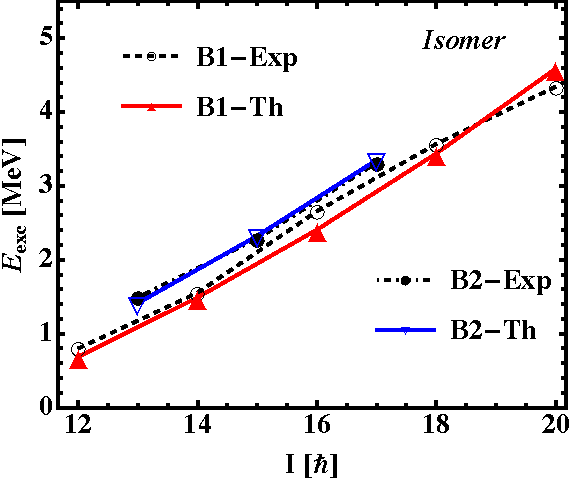
\includegraphics[scale=0.5]{Figs/134Ce-excitation-isomer.pdf}
      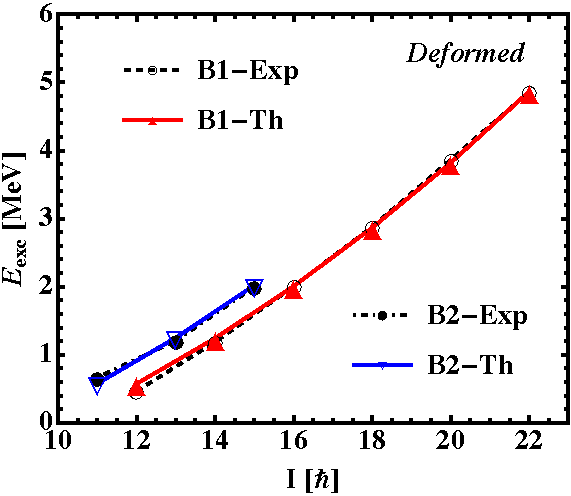
\includegraphics[scale=0.5]{Figs/134Ce-excitation-deformed.pdf}
    \end{figure}
    \item isomer: $\mathcal{J}_1:\mathcal{J}_2:\mathcal{J}_3\to 14:21:\mathbf{34}\ \hbar^2\text{MeV}^{-1}$ 
    \item deformed: $\mathcal{J}_1:\mathcal{J}_2:\mathcal{J}_3\to 15:23:\mathbf{42}\ \hbar^2\text{MeV}^{-1}$
  \end{itemize}
\end{frame}

\begin{frame}
  \frametitle{New Results for 136Nd}
  \begin{columns}
    \begin{column}{0.5\textwidth}
      \begin{figure}
        \centering
        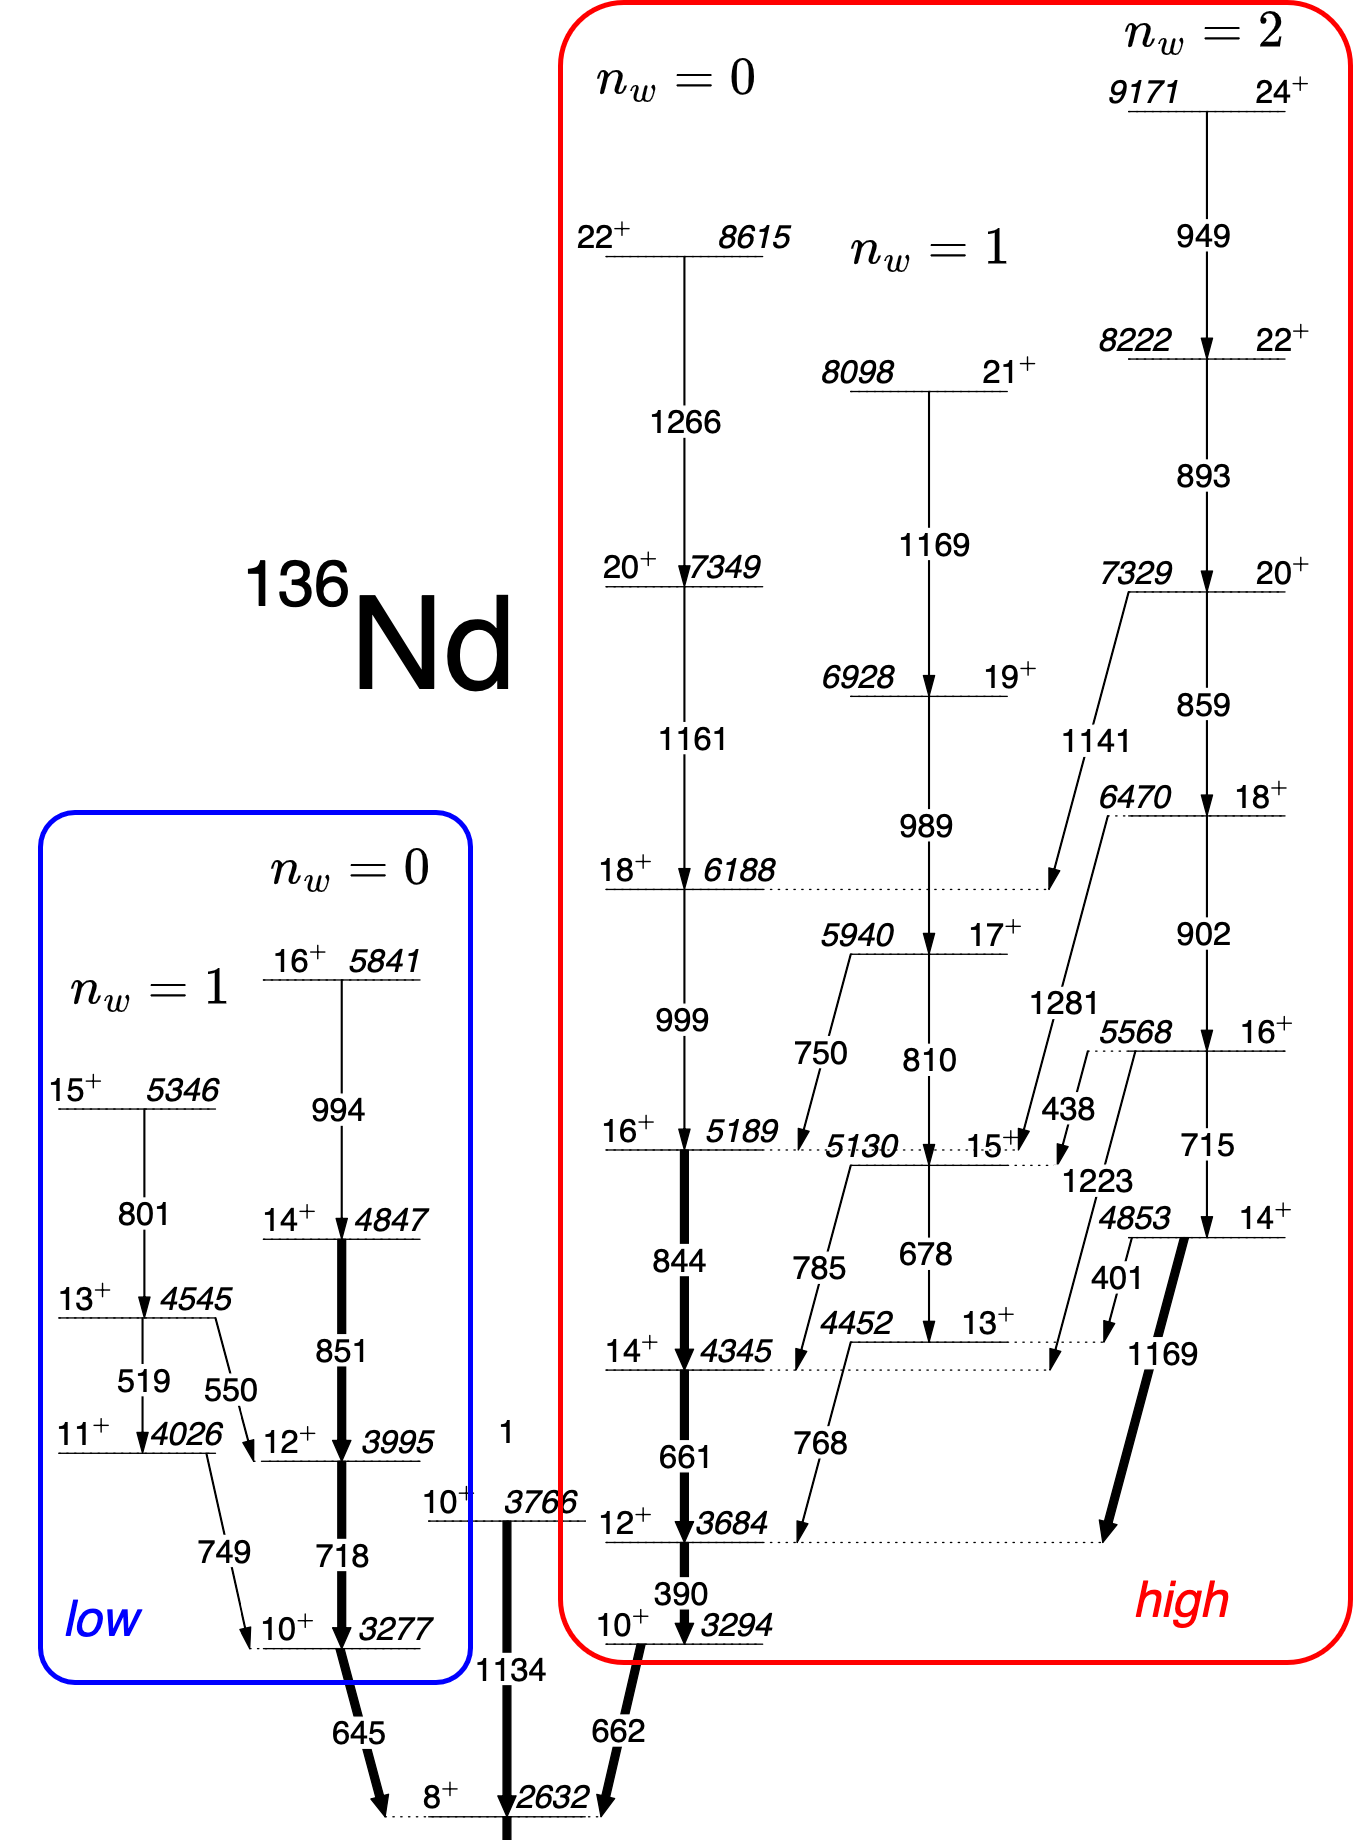
\includegraphics[scale=0.1]{Figs/triaxial-shapes-136Nd.png}
      \end{figure}
    \end{column}
    \begin{column}{0.6\textwidth}
      \begin{itemize}
        \item Lv et al. found two sets of wobbling bands in $^{136}$Nd $\rightarrow$ worth investigating $A=137$ neighbor nuclei ?
        \item \emph{low}/\emph{high} is used to differentiate the energy of $10^+$ state of each structure
        \item The higher structure has two phonon excitations
      \end{itemize}
    \end{column}
  \end{columns}
\end{frame}

\begin{frame}
  \frametitle{New Results for 136Nd II}
\begin{itemize}
  \item Separate fitting for each structure (low/high)
  \item Low: $(\beta,\gamma)=(0.15,-35^\circ)$, $E_\text{RMS}\approx 120$ keV,
  \item High: $(\beta,\gamma)=(0.21,25^\circ)$, $E_\text{RMS}\approx 145$ keV
  \begin{figure}
    \centering
    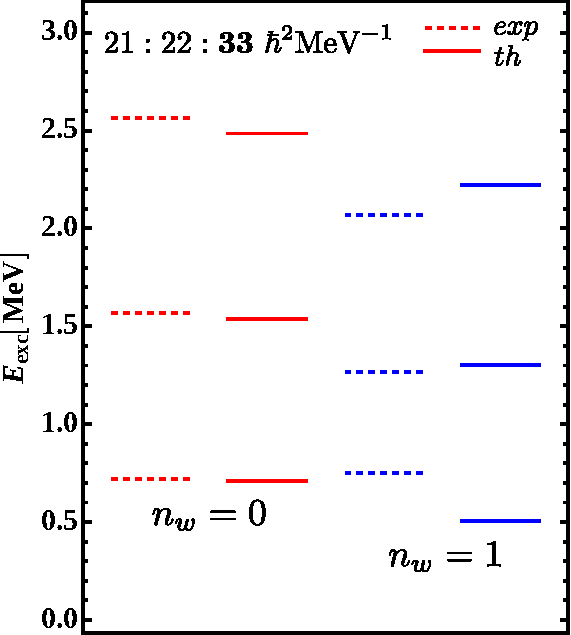
\includegraphics[scale=0.458]{Figs/136Nd-excitation-lower-edited.pdf}
    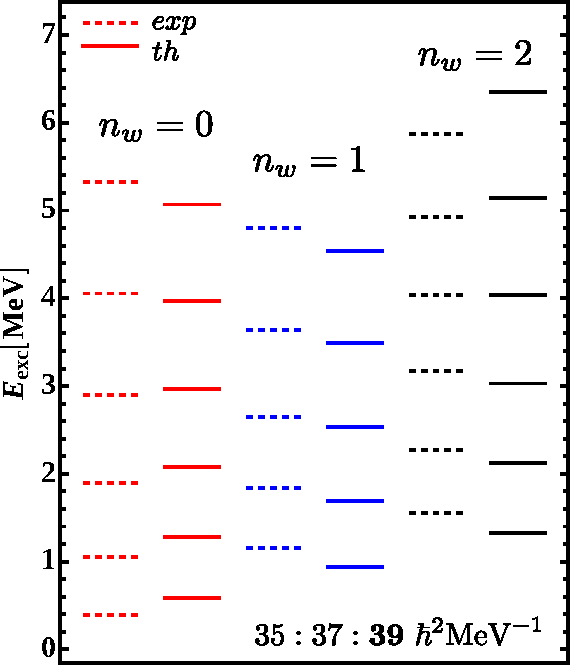
\includegraphics[scale=0.44]{Figs/136Nd-excitation-higher-edited.pdf}
  \end{figure}
\end{itemize}
\end{frame}

\begin{frame}
  \frametitle{Conclusions \& Future Outlook}
  \begin{itemize}
    \item New wobbling nuclei were investigated through a semi-classical formalism
    \item The harmonic approximation reproduces the experimental data of even-$A$ wobbling nuclei
    \begin{itemize}
      \item One wobbling structure for $^{130}$Ba
      \item Two wobbling structures for $^{134}$Ce and $^{136}$Nd 
    \end{itemize}
    \item Quality of the fit was reflected in the transition probabilities for $^{130}$Ba
    \item Calculations were done for fixed deformation parameters
    \item + Employ spin-dependence for the moments of inertia 
    \item + Find classical trajectories $^\text{\tiny\emph{Poenaru R, Raduta A A, IJMPE 2021}}$
  \end{itemize}
\end{frame}

\begin{frame}
  \begin{center}
    \Large Thank you for your attention!
  \end{center}
\end{frame}

%---------------------------------------------------------
\end{document}
%---------------------------------------------------------

